%qqqqqqqqqqqqqqqqqqqqqqqqqqqqqqqqqqqqqqqqqqqqqqqqqqqqqqqqqqqqqqqqqqqqqqqqq
%Quote
\begin{savequote}[50mm]
‘‘All the effects of Nature are only the mathematical consequences of a 
small number of immutable laws’’
\qauthor{Pierre Simon Laplace}
\end{savequote}
%qqqqqqqqqqqqqqqqqqqqqqqqqqqqqqqqqqqqqqqqqqqqqqqqqqqqqqqqqqqqqqqqqqqqqqqqq




%#########################################################################
\chapter{Computational Methods in Cosmology}
\label{cha:N-BodySimulations}


%Reviewed
In recent years, computational physics has acquired an important role in
physics, allowing modelling many high-complexity systems without the
necessity of recurring to experiments and/or observations. Among the methods
covered by computational physics is highlighted the N-body problem since 
many phenomenons require the computation of the interactions between a
large number of bodies. Some illustrative examples of this are the 
modelling of molecular systems, plasma physics and specially gravitational
problems in astrophysics. The development of specific methods to solve 
this type of problems precedes the advent of computer systems, even so, 
their development has powered enormously this discipline such that it is
considered a new branch of physics.


%Reviewed
In this chapter will be covered in detail some specific methods for solving
gravitational problems in astrophysics, specially those related with 
simulations of the large-scale universe in the non-linear regime, ranging 
from basic algorithms to compute forces, methods to detect dark halos, to
basic classification schemes for the cosmological environment.

 

%#########################################################################




%*************************************************************************
%N-body Simulations
\section{N-body Simulations}
\label{sec:N-bodySimulations}


%Reviewed
Generally, the most suitable type of phenomena that can be modelled through 
N-body simulations is those where the interactions are strongly correlated 
between the constituent particles, such as long-range forces or non-local 
interactions. Figure \ref{fig:NbodyProblem} illustrates an arbitrary set 
of point particles which interact each other under the influence of a 
force field $\bds f$. Those conditions shape the classical formulation of 
the N-body problem.


\
%Reviewed
%.........................................................................
%N-Body Problem
\begin{figure}[htbp]
	\centering
	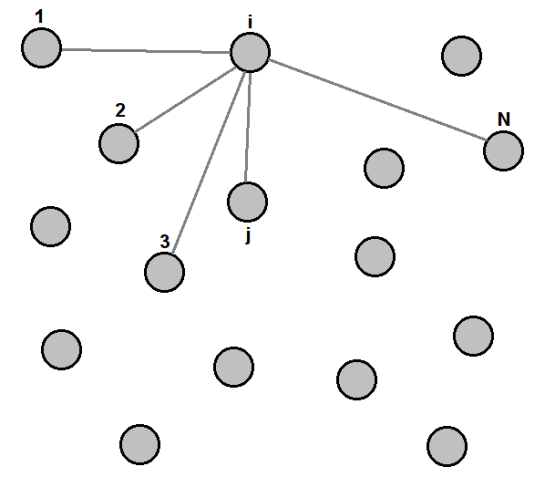
\includegraphics[width=0.50\textwidth]
	{./figures/3_nbody_simulations/Nbody_Problem.png}

	\caption{\small{Formulation of the N-body problem.}}
	
	\label{fig:NbodyProblem}
\end{figure}
%.........................................................................


%Reviewed
Assuming interactions that depends on the position\footnote{ In the 
generalized problem, interactions can depend on other parameters like 
the velocity or intrinsic degrees of freedom like the spin.}, it is 
obtained the below equation of movement of the $i$-th particle shown in 
the Figure \ref{fig:NbodyProblem} \cite{pfalzner1996} \cite{binney2008} 


%Reviewed
%.........................................................................
%Movement Equation
\eq{eq:MovementEquation}
{ \ddot{ \bds r}_i = \sum_{j=1}^N \bds f( \bds r_i, \bds r_j ) = -\nabla 
\phi( \bds r_i )\ \ \ \ \ \ \ i=1,2,\cdots,N }
%.........................................................................
where it has been introduced the potential function $\Phi(\bds r)$. For
the case of gravitational interactions, the potential acquires the form



%.........................................................................
%Gravitational Potential
\eq{eq:GravitationalPotential}
{ \phi(\bds r) = -\sum_{j=1}^N  \frac{G m_j}{|\bds r - \bds r_j|} }
%.........................................................................


%Reviewed
The general solution to the problem is obtained from the set $\{ \bds 
r_1(t),\cdots, \bds r_N(t) \}$, which is determined from the equations
\ref{eq:MovementEquation}. For this it is necessary to implement numerical
approximations due to the non-solvable (analytically) nature of the 
problem.



	%---------------------------------------------------------------------
	%Direct sum
	\subsection{P-P Method}
	\label{subsec:PPMethod}
	%---------------------------------------------------------------------
	
	
%Reviewed
The first approximation to find a solution of the equations of movement
\ref{eq:MovementEquation} is to compute all the $N-1$ interactions of the
$i$-th particle with all of the others in a specific time $t$ and this for
$i=1,2,\cdots N$, then, from a numerical integration scheme it is 
calculated the positions in a discretized later time $t+\Delta t$ and thus
until a given maximum time $t_{\submath{max}}$. This method is called P-P 
(Particle to Particle) and is one of the three standard methods for 
solving the N-body problem.


%Reviewed
When interactions present singularities, such as Coulombic potentials in
electrostatic and gravitational problems (equation 
\ref{eq:GravitationalPotential}), the integration of the equation of 
movement is very sensitive to close encounters between particles and 
therefore the resolution of the time step must be increased, thereby 
implying a considerable increasing of the computing time. A standard 
solution is to introduce a softening parameter that removes these 
singularities, but at the cost of losing accuracy in the solution. For the
gravitational potential \ref{eq:GravitationalPotential}, this leads to


%Reviewed
%.........................................................................
%Gravitational Potential
\eq{eq:SoftPotential}
{ \phi_{s}(\bds r) = -\sum_{j=1}^N  \frac{G m_j}{|\bds r - \bds r_j| 
+ \epsilon_j^2} }
%.........................................................................
where $\epsilon_j$ is the softening parameter and can be interpreted as a
measure of the physical dimension of the particle.


%Reviewed
In spite of the high precision achieved by this method, the computing time
scales as $t_{\submath{comp}}\propto N^2$, what makes it highly non-viable
to apply for a large number of particles (generally $N\gtrsim 10^4-10^5$ 
\cite{padmanabhan1995}). For simulations of planetary systems, computation
of orbits of minor bodies and studies of star clusters dynamics, this 
methods is good enough, but for cosmology and galaxy astrophysics, where 
the number of implicated particles must be the maximum possible in order 
to reproduce the real continuous nature of the matter distribution, it 
becomes necessary to develop methods lesser computational 
cost.



	%---------------------------------------------------------------------
	%Tree codes
	\subsection{PM Method}
	\label{subsec:PMMethod}
	%---------------------------------------------------------------------
	
	
%Reviewed
A second scheme used for solving the N-body problem is the PM scheme 
(Particle Mesh) \cite{dawson1983}, this consists of determining a 
continuous distribution for the density field from the position and the
mass value of each particle, for this it is divided the space of the 
simulation into a grid of $M\times M\times M$ cells and then a count of
particles per cell is made in order to associate a specific mass value and
therefore a density to each cell. An illustrative diagram is shown in 
Figure \ref{fig:MP_Method}


%Reviewed
%.........................................................................
%PM Method
\begin{figure}[htbp]
	\centering
	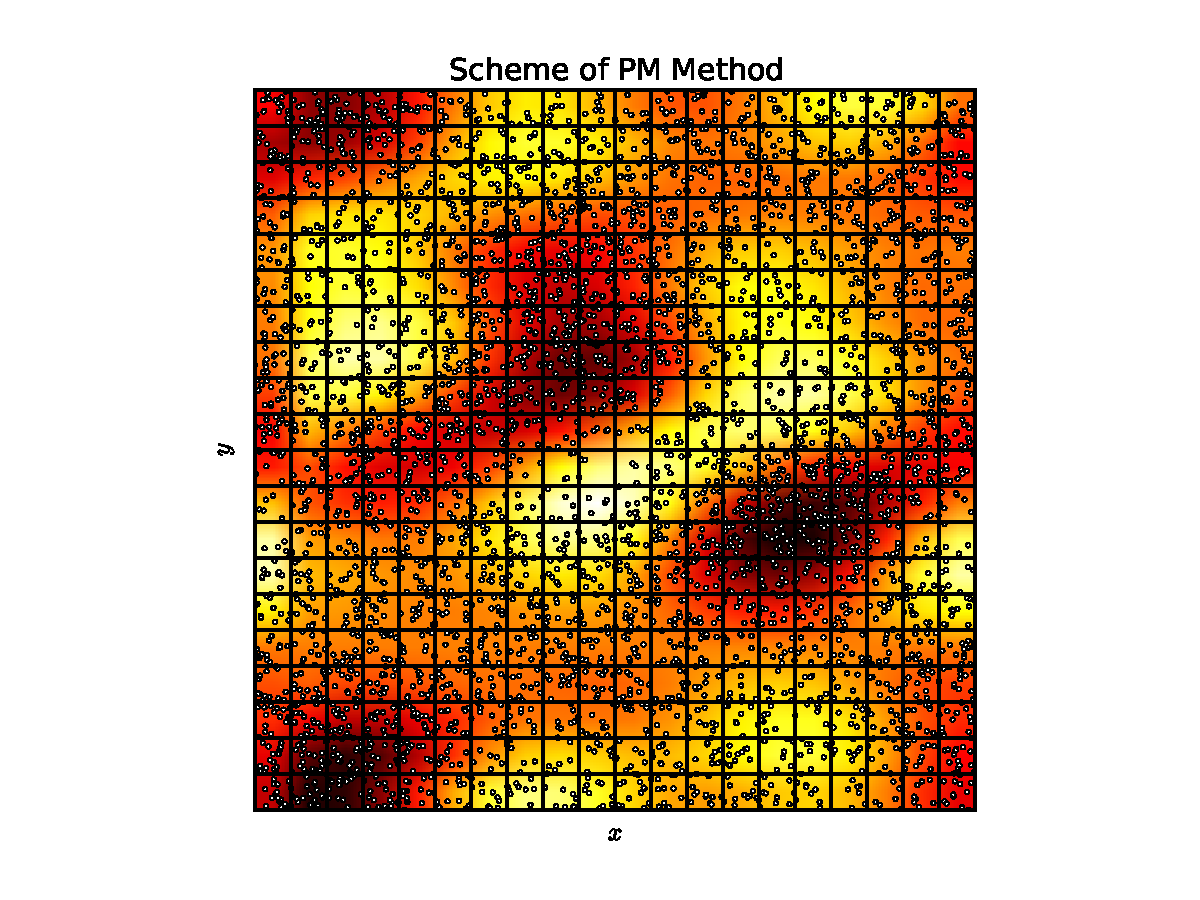
\includegraphics[width=1.00\textwidth]
	{./figures/3_nbody_simulations/PM_Method.pdf}

	\caption{\small{Illustrative diagram of the PM method. The map that is
	plotted over the distribution of particles corresponds to the density
	field evaluated in each cell of the grid. Dark cells corresponds to
	overdensity regions whereas white cells to lower values of the density 
	field, which agrees with the amount of mass of the particles per cell.}}
	
	\label{fig:MP_Method}
\end{figure}
%.........................................................................
%Reviewed
\newpage
The method can be summarized into the next steps


%Reviewed
%.........................................................................
%Particle Mesh steps
\begin{itemize}
\item[\textbf{1.}] From the grid established over all the simulation, it
is calculated a continuous density field $\rho(\bds r)$, interpolating the
value between adjacent cells.

%Reviewed
\item[\textbf{2.}] Once it is obtained the density field, it is calculated
the potential of the equation of movement \ref{eq:MovementEquation} by 
using the Poisson's equation



%.........................................................................
%Poisson Equation
\eq{eq:Poisson}
{ \nabla^2 \phi = 4 \pi G \rho }
%.........................................................................


%Reviewed
In order to reach this, it is usually used integration schemes based upon
Fourier transform, such as the Fast Fourier Transform (FFT).


%Reviewed
\item[\textbf{3.}] Finally, using the previous potential field, it is 
calculated the position of each particle in the next discrete time
$t+\Delta t$, and it is repeated over and over again until a given
final time.
\end{itemize}
%.........................................................................


%Reviewed
This method is less precise than the direct sum, but it is possible to 
demonstrate that the computing time scales as $t_{\submath{comp}} 
\propto N + M \log M$, with an asymptotic behaviour as $t_{\submath{comp}} 
\propto N$ for high resolutions $M$ of the grid and as $t_{\submath{comp}} 
\propto N$ for low resolutions \cite{pfalzner1996}. In any case, its 
efficiency is much better than the PP method \ref{subsec:PPMethod} when
the number of particles of the simulation is large enough $N\ll 10^4 - 
10^5$, which makes this method very useful to tackle problems with a large
number of particles.


%Reviewed
However, there are some pathological situations where this method can not
be applied satisfactory \cite{pfalzner1996}.


%Reviewed
%.........................................................................
%Difficulties of PM Method
\begin{itemize}
\item Highly non-homogeneous distributions of particles.
\item Strongly correlated systems.
\item Systems with non-trivial geometries.
\end{itemize}
%.........................................................................


%Reviewed
Because those conditions are satisfied in the non-linear universe, like 
strong gravitational couplings for modes of the density field after 
$z\gtrsim 8$, this methods is not very useful for solving the late 
universe.



	%---------------------------------------------------------------------
	%Hidrodynamical and dark matter simulations
	\subsection{P$^3$M Method}
	\label{subsec:P3Method}
	%---------------------------------------------------------------------
	
	
%Reviewed
The last of the three standard scheme for solving N-body simulations is 
the P$^3$M method (PP $+$ PM) \cite{hockney1988}. This method can be 
thought as a combination of the previous methods, making the most of each
one of them.


%Reviewed
%.........................................................................
%P3M Method
\begin{figure}[htbp]
	\centering
	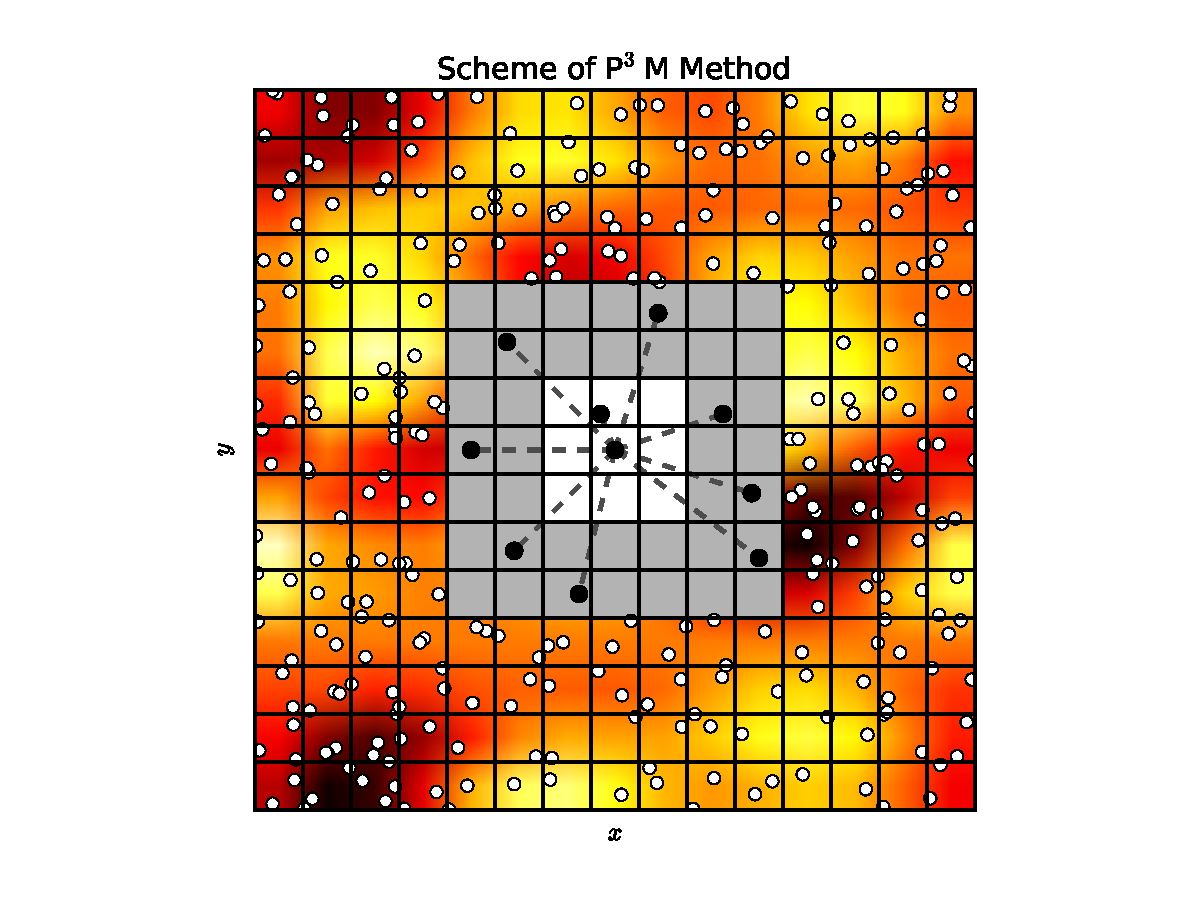
\includegraphics[width=1.00\textwidth]
	{./figures/3_nbody_simulations/P3M_Method.pdf}

	\caption{\small{Illustrative diagram of the P$^3$M method. For the 
	reference particle, shown in the center, interactions with distant 
	particles is calculated through the PM method, whereas for close
	particles (gray and white regions), the interaction is calculated 
	by using the PP method.}}
	
	\label{fig:P3M_Method}
\end{figure}
%.........................................................................


%Reviewed
Figure \ref{fig:P3M_Method} illustrates the P$^3$M method. For each one of
the integration step of the system, it is calculated a hierarchical grid 
for each particle. Hierarchies are defined with respect to the relative
distance between particles and they determines which approximation should
be used for computing the equation of movement. For close particles (first
hierarchy) it is used the PP method, what allows tackling strong local 
correlations and highly non-homogeneous regions. Interactions with 
particles embedded into the next hierarchies are calculated by decomposing 
the potential field into its multipolar terms, i.e. the second hierarchy
corresponds to the dipolar contribution of the potential (if applicable), 
and so on. Finally for more distant cells (last hierarchy), it is used the
PM scheme, interpolating the density field and solving the Poisson's 
equation \ref{eq:Poisson} for the potential.


%Reviewed
%.........................................................................
%Tree Code Building
\begin{figure}[htbp]
	\centering
	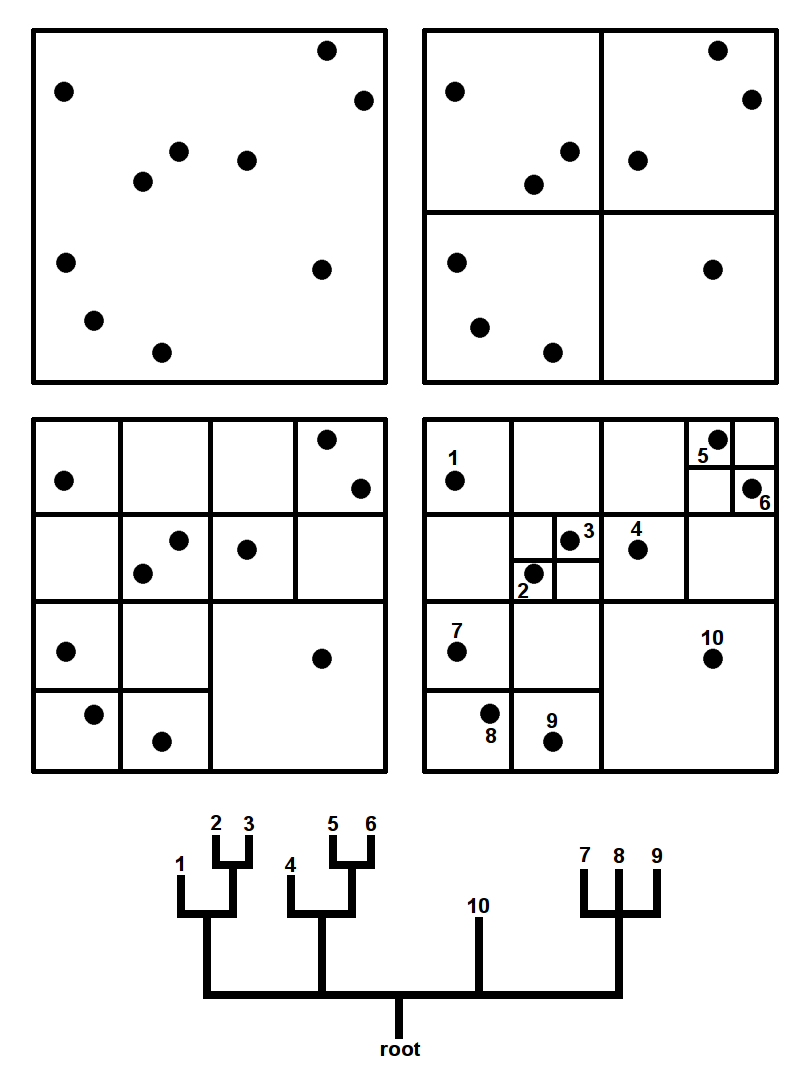
\includegraphics[width=0.72\textwidth]
	{./figures/3_nbody_simulations/TreeCode.png}

	\caption{\small{An illustrative example of the building of a tree code
	for a N-body simulation. Upper panels show the iterations for a 2D 
	problem whereas lower panel illustrates the resultant tree built using 
	each particle of the simulation.}}
	
	\label{fig:Tree_Code}
\end{figure}
%.........................................................................
\newpage


%Reviewed
One of the main disadvantages of this method lies in the building of the
hierarchical structure for evaluating which scheme must be used. The 
original scheme, proposed simultaneously by \cite{appel1985} 
\cite{jernigan1985} and \cite{porter1985}, has some inconsistencies 
produced by the lack of physical basis in the building of the hierarchical
structure \cite{pfalzner1996}.


%Reviewed
A better physically based method for constructing the hierarchical 
structure of a N-body simulation is the so-called octant tree code. It was
initially developed by \cite{barnes1986}. In this algorithm, the space of 
the simulation is embedded into a cubic volume denominated \textit{root},
then this volume is divided into 8 regions of equal size which are 
denominated octant, these are the first hierarchy of the tree. This 
procedure is repeated recursively until each cell or octant has only one
particle inside, thereby constructing a set of hierarchies that determines
the neighbourhood of all the particles of the simulation. Figure 
\ref{fig:Tree_Code} illustrates the iterations needed in order to construct
the tree of a simulation (with the aim of simplicity, it is 2D). The lower
panel of the same figure shows the structure of the tree. In this way it
is possible to compute, for instance, the interaction between particles 7,
8 and 9 by using direct sum, because they are the closer neighbours each 
other, whereas the interaction with other particles that belong to other 
branches is calculated through multipolar expansion or the PM scheme.



%*************************************************************************




%*************************************************************************
%Types of simulations
\section{Types of Simulations}
\label{sec:Types of Simulations}


%Reviewed
Using the methods above described, it is possible to carry out simulations
of the late universe in the non-linear regime and studying its behaviour 
numerically. Because in the non-linear regime all the large-scale 
astrophysical processes are dominated mainly by dark matter, it is usual 
not considering the contribution of other components like radiation or 
baryonic matter, furthermore, including the different physical processes
dominated by these other contributions would increase considerably the 
computing time of the simulation without much profit regarding physical
understanding. This specific type of simulations is called \textit{dark 
matter simulations}.


%Reviewed
In this subsection are shown the dark matter simulations that are used
throughout this work, moreover they are classified with respect to the
adopted criterion for setting the initial conditions, thus, simulations
can be unconstrained when the initial conditions are set in a completely 
random way, or constrained when they are chosen such that they satisfy 
some conditions fixed a priori like observational constraints or 
reproducing the very local structure ($\sim 10$ Mpc$/h$) of the real 
universe.


	%---------------------------------------------------------------------
	%Unconstrained simulations (Bolshoi)
	\subsection{Unconstrained Simulations (Bolshoi)}
	\label{subsec:UnconstrainedSimulations}
	%---------------------------------------------------------------------


%Reviewed
Since the evolution of the universe in the linear regime is well-know 
through the transfer function (see section 
\ref{sec:LinearStructureFormation}), dark matter cosmological simulations 
are only used for studying the non-linear regime, however it is necessary 
to establish a set of initial conditions in order to evolve the system 
properly. Generally these conditions are determined from computing the 
linear regime, so that it is required another set of primordial conditions 
for the homogeneous background density field. Because of that, the last 
set will be henceforth called simply the initial conditions.


%Reviewed
As has been mentioned in the subsection \ref{subsec:StatisticalProperties},
the statistical properties of the initial density field correspond to a
Gaussian distribution of the Fourier modes with a Harrison-Zeldovich 
power spectrum, which agrees with the inflationary model and cosmological
observations (see subsection \ref{sec:CosmologicalObservations}). The 
modes of the density field $\delta_{\bds k} = r_{\bds k}e^{i\phi_{\bds k}}$
follow then the distributions given by the equation 
\ref{eq:GaussianDistribution}



%.........................................................................
%Radial distribution
\eq{eq:RadialModeDistribution}
{ P_r(r_{\bds k})dr_{\bds k} = \exp\pr{ -\frac{r_{\bds k}^2}{\sigma_k^2} }
\frac{2r_{\bds k}dr_{\bds k}}{\sigma_k^2} }
%.........................................................................


%.........................................................................
%Angular distribution
\eq{eq:PhiModeDistribution}
{ P_\phi(\phi_{\bds k})d\phi_{\bds k} = \pr{\frac{1}{2\pi}}d\phi_{\bds k} }
%.........................................................................


%Reviewed
The unconstrained nature of this type of simulations lies in the 
randomness of the phases $\phi_{\bds k}$ according to the distribution
\ref{eq:PhiModeDistribution}, without any kind of observational 
constrained for the final stage of the simulation.


\
%Reviewed
\textbf{\textit{Bolshoi}} is a cosmological simulation of the large-scale
universe with unconstrained initial conditions, the official website of
the project is \url{http://hipacc.ucsc.edu/Bolshoi/}. 

\newpage
%Reviewed
%.........................................................................
%Bolshoi Simulation Evolution
\begin{figure}
	\centering
	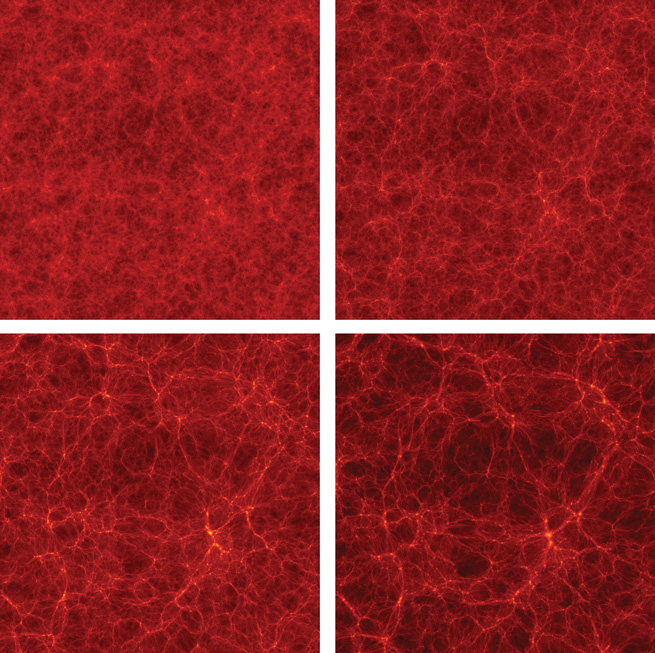
\includegraphics[width=0.80\textwidth]
	{./figures/3_nbody_simulations/Bolshoi_Evolution.png}

	\caption{\small{Evolution of the Bolshoi simulation. It is illustrated
	the density field in a rectangular volume of $16$ Mpc$/h$ of thick and
	$250$ Mpc$/h$ of side for different stages of the evolution. $z=9.5$ 
	(upper left), $z=3$ (upper right), $z=1$ (lower left) y $z=0$ (lower
	right). Taken from 
	\url{http://spectrum.ieee.org/aerospace/astrophysics/the-cosmological-supercomputer} }}
	
	\label{fig:Bolshoi_Evolution}
\end{figure}
%.........................................................................


%Reviewed
Due to its larger comoving size compared to constrained simulations (a
cubic volume of $250$ Mpc$/h$), Bolshoi is used for obtaining the 
fine-grained statistics for the results computed in the chapter
\ref{cha:Results}. The cosmological model used in this simulation is the 
WMAP7 universe (see Table \ref{tab:CosmologicalParameters}), the number of
particles used is $2048^3$, what implies a mean mass per particle of 
$1.35 \times 10^8 h^{-1}$ M$_{\odot}$. More precise and technical 
information about can be consulted in \cite{klypin2011}.
\newpage



	%---------------------------------------------------------------------
	%Constrained simulations (CLUES)
	\subsection{Constrained Simulations (CLUES)}
	\label{subsec:ConstrainedSimulations}
	%---------------------------------------------------------------------


%Reviewed
As has been mentioned in the chapter \ref{cha:Theoretical Framework}, the
standard way to compare the results produced by cosmological simulations 
and observations is through the statistical properties of the 
distributions, such as the two-point correlation functions or the power 
spectrum. In spite of that, some studies require more detailed description
of the local universe in a cosmological context. Due to technical issues, 
like the direct measuring of the dark matter distribution or the lack of 
data in high redshifts, it is necessary to appeal to cosmological 
simulations that reproduce properly the local universe. One of the first 
work aimed to reproduce the local universe is \cite{Klypin2003}. Here it 
is reproduced our local group of galaxies along with the local 
supercluster and the Virgo cluster.


%Reviewed
%.........................................................................
%Constrained Simulation
\begin{figure}[htbp]
	\centering
	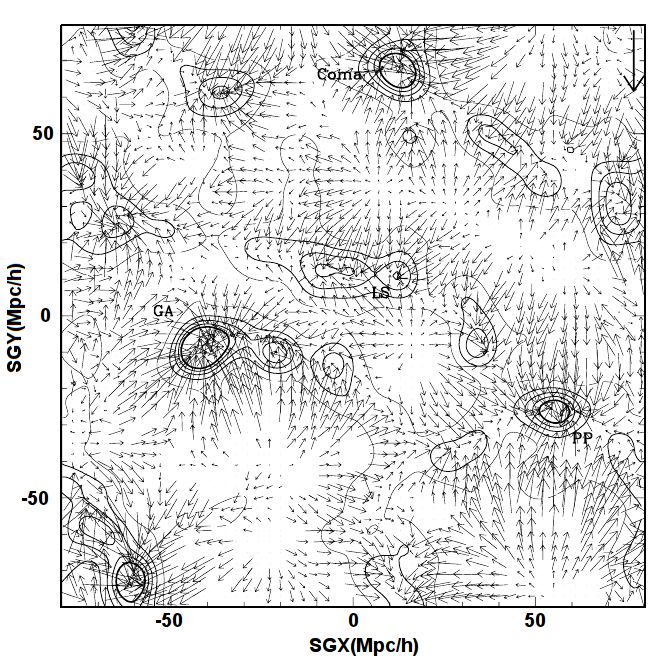
\includegraphics[width=0.70\textwidth]
	{./figures/3_nbody_simulations/Constrained_Construction.png}

	\caption{\small{Initial density and peculiar velocity field built by 
	using constraints in order to reproduce the local environment at a 
	scale of $160\ h^{-1}$Mpc. Some of the identified structures are:
	\textit{Coma}, coma cluster, \textit{PP}, Perseus-Pisces supercluster,
	\textit{LS}, local supercluster, \textit{GA}, the great attractor. 
	The upper arrow indicates the scale of the peculiar velocities field 
	as $1000$ km/s. Taken from \cite{Klypin2003}.}}
	
	\label{fig:Constrained_Construction}
\end{figure}
%.........................................................................


%Reviewed
The method proposed by \cite{Klypin2003} and \cite{Hoffman1991} consists in
building the initial density and peculiar velocities field from surveys of 
radial velocities and redshifts (see section 
\ref{sec:CosmologicalObservations}). For the treatment and reduction of 
noise and measuring errors of data, it is used a Bayesian method, 
Wiener filters (for more detailed information, see \cite{Zaroubi1999}).
At small scales, this method is limited because the applied filters 
suppress some modes in the initial power spectrum and therefore they must
be generated randomly according to the Gaussian distribution 
\ref{eq:GaussianDistribution} in order to guarantee consistency with the
standard cosmological model. Figure \ref{fig:Constrained_Construction} 
illustrates the initial conditions obtained by this method for the local
universe at a scale of $160\ h^{-1}$Mpc.


%Reviewed
%.........................................................................
%CLUES Right Simulation
\begin{figure}[htbp]
	\centering
	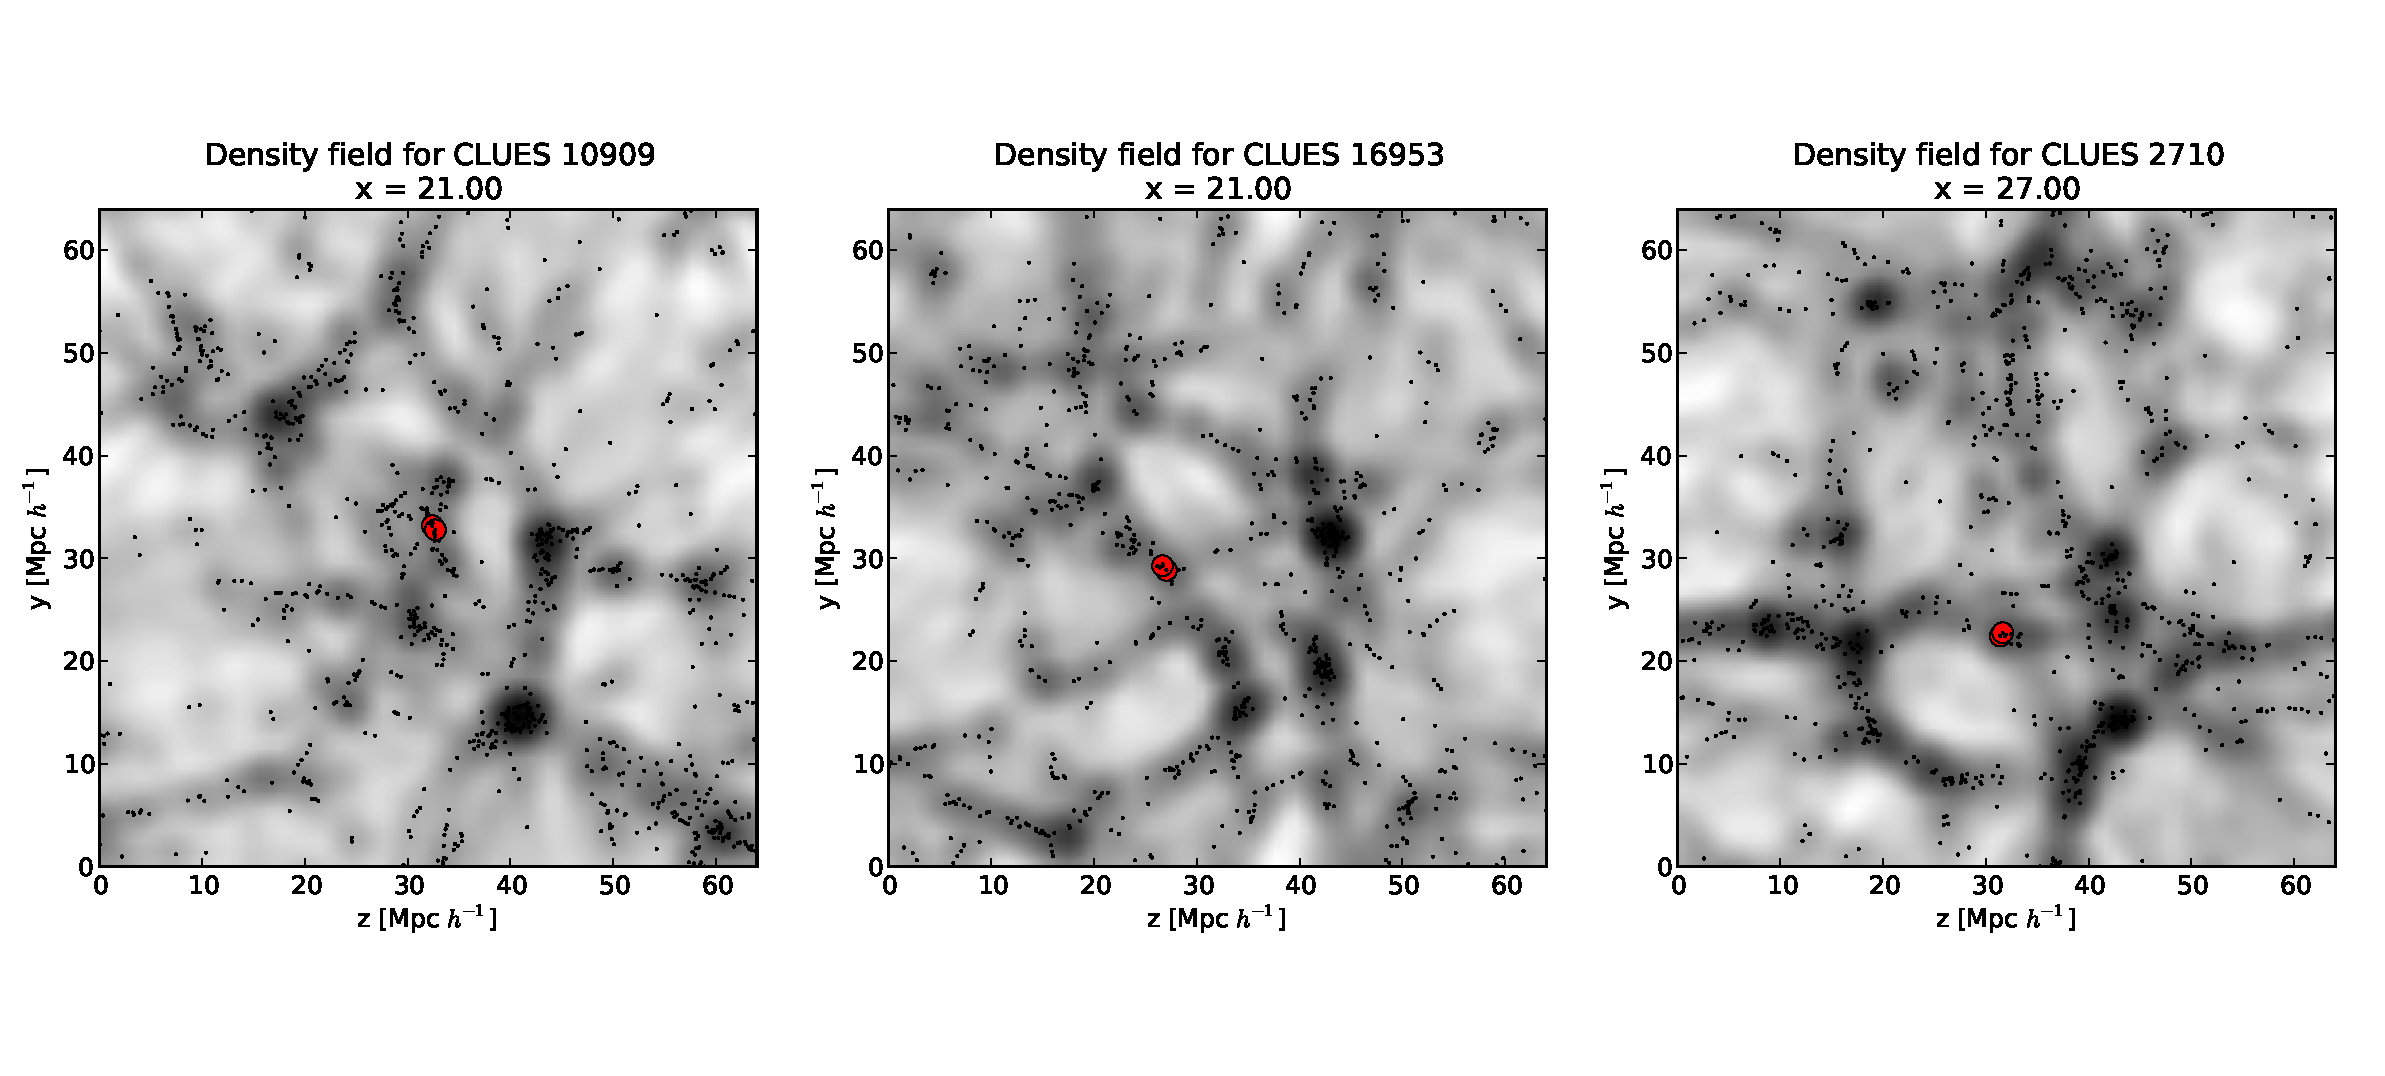
\includegraphics[width=1.0\textwidth]
	{./figures/3_nbody_simulations/CLUES_Simulations.pdf}

	\caption{\small{Three constrained simulations of the CLUES project 
	where it is possible to identify systems like the local group. It is
	illustrated the density field of each simulations along with the dark
	matter halos (black points), and the LG-like systems found (red 
	points).}}
	
	\label{fig:CLUES_Right}
\end{figure}
%.........................................................................


%Reviewed
\textbf{CLUES} (Constrained Local UniversE Simulations) is a project aimed
to reproduce the local universe with the best resolution up to date. The 
official webpage of the project is \url{http://www.clues-project.org}. In 
this simulations, initial conditions are built by using the Hoffman-Ribak
algorithm \cite{Hoffman1991} for reproducing a comoving volume of $(64\ 
h^{-1}$Mpc$)^{3}$. Due to the unconstrained nature of initial conditions at
small scales ($\sim 5\ h^{-1}$Mpc), it becomes necessary to carry out $200$
different simulations, of which only $3$ are successful regarding the 
imposed observational constraints (see Figure \ref{fig:CLUES_Right}).
For the evolution it is used the package \texttt{GADGET2}\footnote{
\texttt{GADGET2} is a very popular code for N-body simulations developed
by Volker Springel. It is available for free download in the official 
webpage of the project \url{http://www.mpa-garching.mpg.de/gadget/}}
with $1024^3$ particles of dark matter and a cosmology consistent with
the WMAP7 (see Table \ref{tab:CosmologicalParameters}). More technical 
details  and further information of the project can be found in
\cite{Gottloeber2010}.


%Reviewed
%.........................................................................
%CLUES Simulation Overview
\begin{figure}[htbp]
	\centering
	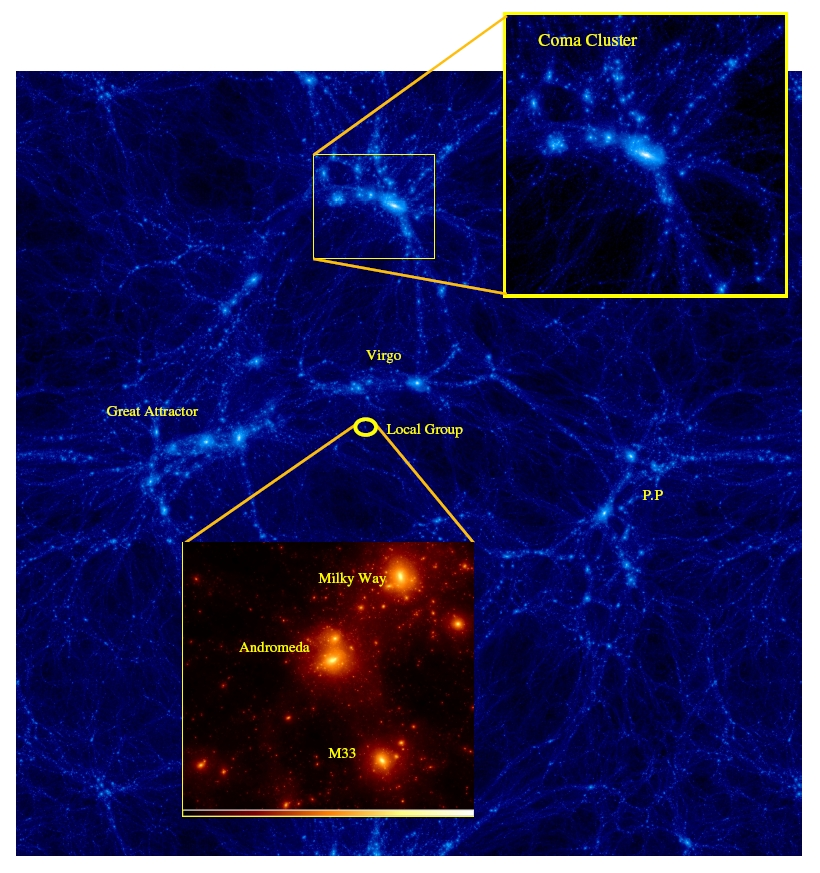
\includegraphics[width=0.90\textwidth]
	{./figures/3_nbody_simulations/CLUES_Overview.png}

	\caption{\small{An example of a simulation of the CLUES project. In 
	this figure it is shown the large-scale structures of the local 
	universe and it can be appreciated clearly the most significant members
	of the Local Group. Taken from the official webpage of the project
	\url{http://www.clues-project.org}}}
	
	\label{fig:CLUES_Overview}
\end{figure}
%.........................................................................



%*************************************************************************



%*************************************************************************
%Environment Characterization
\section{Environment Characterization}
\label{sec:EnvironmentCharacterization}


%Reviewed
Once obtained the numerical simulations for the evolution of the universe 
in non-linear regime, one of the main objectives is to characterize the 
emergent structures typical of this regime. Among these structures, it is
highlighted the cosmic web, which is constituted by regions of different 
dimensionality, where vast void regions are limited by planar regions, 
these are, in turn, limited by one-dimensional filaments which joint to 
form high density point regions.


%Reviewed
From cosmological observations, it has been possible to establish the 
relation between the properties of halos, such as the spin parameter, the
concentration, the shape, etc. And the host environment. Because of this,
it is important to quantify the structure of the cosmic web in cosmological
simulations. One of the pioneer works in quantifying the cosmic web was 
the Zeldovich approximations discussed in subsection 
\ref{subsec:Zeldovich'sApproximation}), later schemes use stratifications
in the density field in order to quantify the environment, these schemes
are called geometric methods, but due to their local nature, they cannot
give account of global properties like large-scale matter streams or the
influence of large neighbouring structures. In this section is shown two
recently developed classification schemes.



	%---------------------------------------------------------------------
	%The T-web Method
	\subsection{T-web Scheme}
	\label{subsec:TheT-webMethod}
	%---------------------------------------------------------------------


%Reviewed
The first of these methods was proposed by \cite{Hahn2007} and it consists
in using the theory of dynamical systems in order to perform an analysis
of the local stability of test orbits around dark matter halos, thereby
quantifying their environment for a set time (or set redshift). For this,
the Newtonian approximation is assumed to be correct (see subsection 
\ref{subsec:Newtonian Approximation}) and the equation of movement of a 
test particle embedded into a peculiar potential of the distribution is



%.........................................................................
%Equation of Movement 
\eq{eq:Tweb_Movement}
{ \ddot{\bds r} = - \nabla \phi(\bds r) \ \ \ \ 
\mbox{con}\ \ \ \ \ \nabla^2 \phi = 4\pi G \bar \rho \delta}
%.........................................................................


%Reviewed
It is reasonable to assume that in the center of mass $\bar{\bds r}_i$ of 
each halo there is a minimum of the potential, i.e. $\nabla \phi = 0$, 
thereby forming a local potential well. This allows linearizing the 
equation of movement \ref{eq:Tweb_Movement} around these points, obtaining


%Reviewed
%.........................................................................
%Lineal Equation of Movement 
\eq{eq:Lineal_Tweb}
{ \ddot{r}_i = - T_{ij}(\bar{\bds r}_i)( r_j - \bar{ r}_{k,j})}
%.........................................................................
where it is defined the tidal tensor as the Hessian matrix of the peculiar
potential



%.........................................................................
%Tweb Tensor
\eq{eq:Tweb_Definition}
{ T_{ij} \equiv \frac{\partial^2 \phi}{\partial r_i \partial r_j}}
%.........................................................................


%Reviewed
According the theory of dynamical systems, a negative eigenvalue 
indicates an unstable point in the direction of the respective eigenvector, 
thereby implying an outward flux of matter. For positive eigenvalues, it is
presented a completely analogous situation. Base upon the Zeldovich 
approximation (see subsection \ref{subsec:Zeldovich'sApproximation}), it is
proposed a classification scheme for the cosmological environment from the
eigenvalues of the tidal tensor $T_{ij}$ 
(see Figure\ref{fig:ClassificationSchemeTweb}). 


%Reviewed
%.........................................................................
%Classification of Cosmological Environment
\begin{itemize}
\item \textbf{Vacuum:} in this case, the three eigenvalues are positive,
thereby indicating an expansion into all directions of space.
\item \textbf{Sheet:} in this case $\lambda_1\geq\lambda_2>0$ and 
$\lambda_3<0$, thereby implying an one-dimensional collapse, and leading 
to a region with a planar local geometry.
\item \textbf{Filament:} for this type of regions, only the value of 
$\lambda_1$ is positive, implying a collapse into two directions and an 
expansion into the other one, thereby forming a region with a linear 
geometry.
\item \textbf{Knot:} finally, for this type of region, the three 
eigenvalues are negative, so there is a collapse into all the directions,
leading a highly compressed zone.
\end{itemize}
%.........................................................................


%Reviewed
The most remarkable of this scheme compared to geometric methods is
its dynamical nature, since it allows differentiating regions with the 
same density value but with different stability properties. In spite of
the latter, assuming a local minimum is only justified in the center of
each halo, therefore it is meaningless to generalize this scheme for any
other region of the space. Another inconvenient is that, according to the
original scheme, using the sign of each eigenvalue instead of using the
threshold value, it is not reproduced the visual impression obtained 
from the dark matter distribution of the simulations (see Figure
\ref{fig:TwebVwebComparison}).


%Reviewed
%.........................................................................
%Classification Scheme
\begin{figure}[htbp]
	\centering
	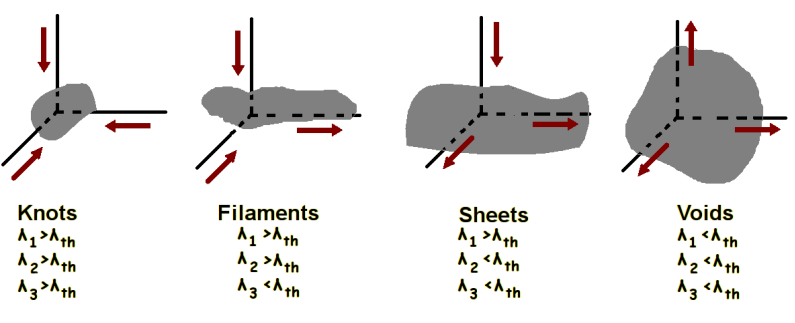
\includegraphics[width=0.9\textwidth]
	{./figures/2_theoretical_framework/EnvironmentClassification.png}

	\caption{\small{Classification scheme for the cosmological environment for
	both T-web and V-web schemes. The threshold value $\lambda_{th}$ is taken as
	free parameter.}}
	
	\label{fig:ClassificationSchemeTweb}
\end{figure}
%.........................................................................



%Reviewed
A significant improvement of this method is reached by generalizing the
classification scheme respect to a certain threshold value $\lambda_{th}^T$,
which is taken as a free parameter and is adjusted according to the visual 
impression obtained \cite{forero2008}. Specially, the original scheme is 
recovery by setting $\lambda_{th}^T=0$.



	%---------------------------------------------------------------------
	%The V-web Method
	\subsection{V-web Scheme}
	\label{subsec:TheV-webMethod}
	%---------------------------------------------------------------------


%Reviewed
The second dynamical scheme to classify the cosmic web presented in this 
chapter is due to \cite{hoffman2012} and it is based upon the peculiar 
shear velocity tensor


%Reviewed
%.........................................................................
%Vweb Tensor
\eq{eq:Vweb_Definition}
{ \Sigma_{ij} = -\frac{1}{2 H_0}\pr{ \der{v_i}{r_j} + \der{v_j}{r_i} } }
%.........................................................................
analogously to the T-web scheme, the eigenvalues of the tensor $\Sigma_{ij}$
are calculated and the environment is defined according to a threshold 
value $\lambda_{th}^V$ (see Figure \ref{fig:ClassificationSchemeTweb}).


%Reviewed
As it has been demonstrated by \cite{hoffman2012}, in the linear regime 
both tensors $T_{ij}$ and $\Sigma_{ij}$ are proportional, therefore both
schemes are completely equivalent in this time. This fact is partially 
evidenced through the visual impression obtained for both schemes from
the large-scale structure in the Bolshoi simulation (see Figure
\ref{fig:TwebVwebComparison}), and that is due to the linearity of
individual Fourier modes at very large scales.


%Reviewed
%.........................................................................
%Tweb Vweb Comparison
\begin{figure}[htbp]
	\begin{center}
	\makebox[\textwidth]{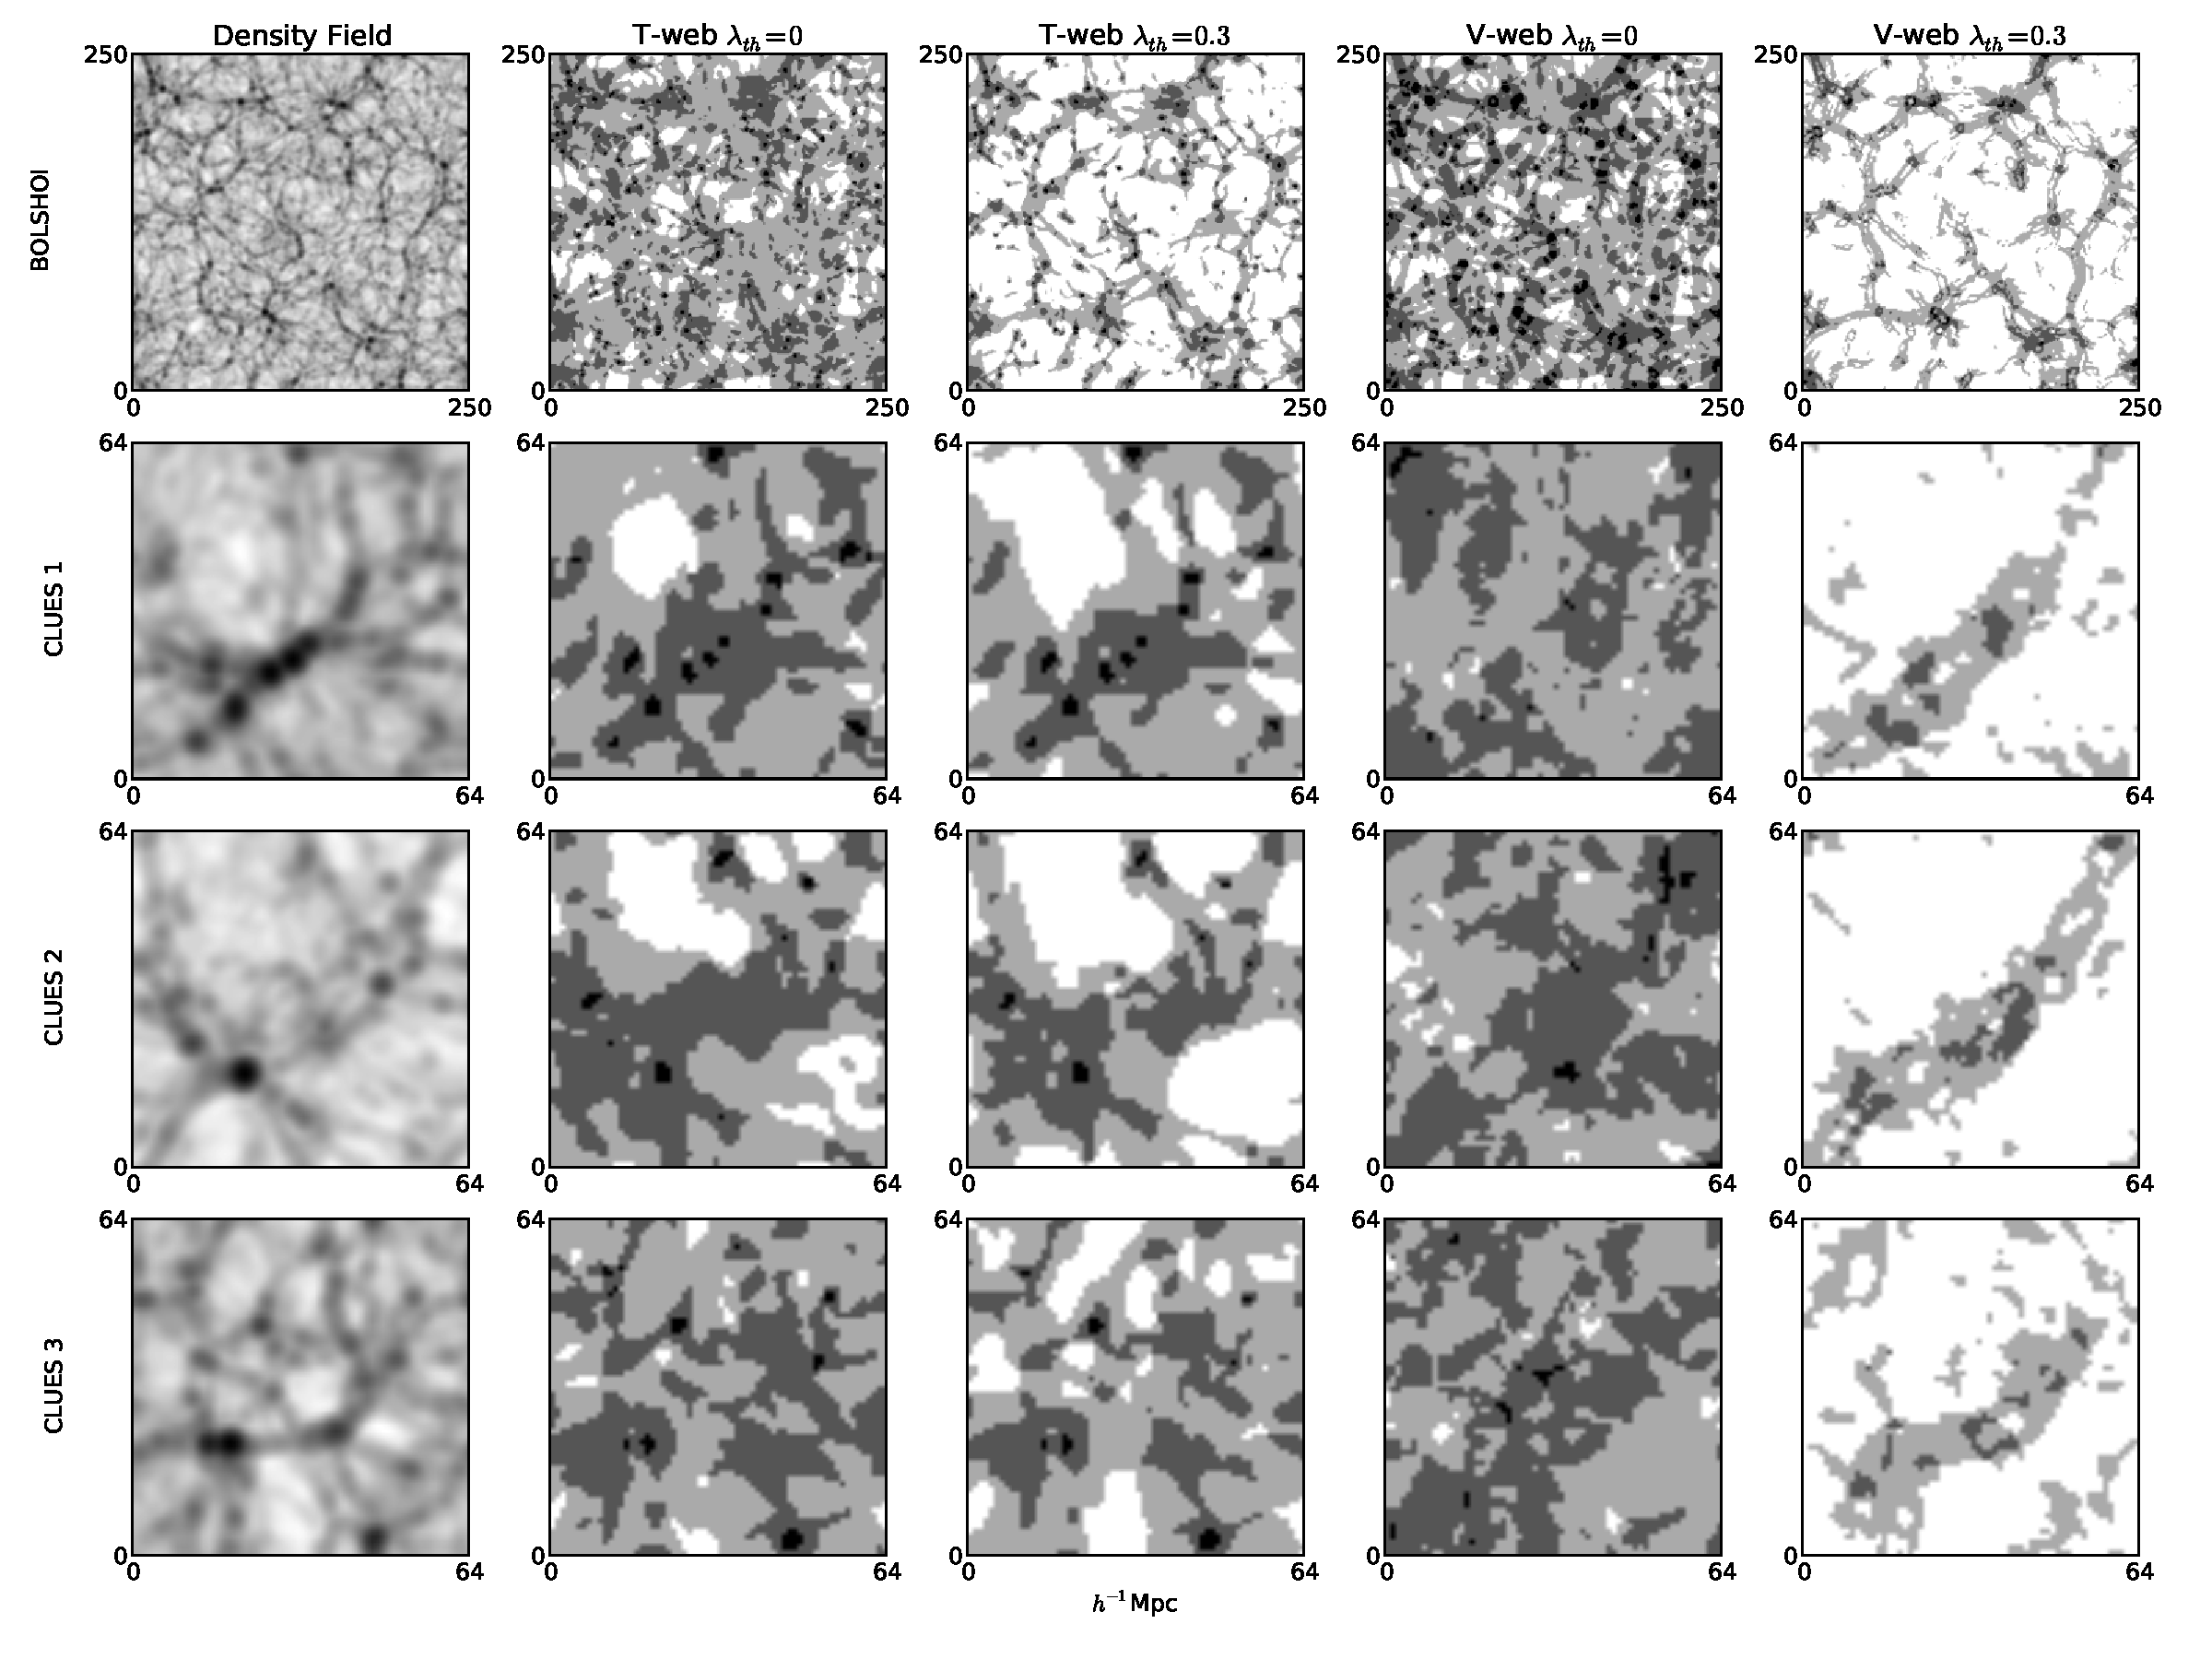
\includegraphics[trim = 5mm 8mm 10mm 5mm, clip, 
	width=0.80\paperwidth,angle=-90]
	{./figures/3_nbody_simulations/Vweb_Tweb.pdf}}
	\end{center}

	\caption{\small{It is illustrated for each one of the simulations
	(CLUES 1, CLUES 2, CLUES 3, Bolshoi) the difference between both 
	classification schemes, T-web and V-web, and for different threshold
	values $\lambda_{th}$ (Black - Knot, Dark gray - Filament, Gray - Sheet,
	White - Vacuum). In the upper figures it is shown the visual impression
	obtained from the respective density fields ($\log (\delta+1)$), these
	impressions are used to calibrate the threshold value $\lambda_{th}$.
	The resolution of the used grid in each simulation is approximately 
	$1.0 h^{-1}$ Mpc/cell and for each one it is performed a Gaussian 
	softening of one cell size. The width of each slide is one cell.}}
	
	\label{fig:TwebVwebComparison}
\end{figure}
%.........................................................................


%Reviewed
For small modes, where non-linear effects are more dominant, both schemes
differ significantly, as it can be seen in the visual impression of
the CLUES simulations. Specifically, the V-web scheme quantifies in a more
precise way the fine structure of the cosmic web at small scales, thereby 
allowing defining a more appropriate environment for cosmologically small 
structures like dark matter halos or small groups of them.


%Reviewed
Another advantage of the V-web scheme regarding the T-web is because the 
V-web is based upon the shear velocity field instead of the density field, 
thereby giving more information about the dynamic of the local environment
and making possible to quantify more directly non-local effects, like fluxes
of matter or the influence of neighbour structures. Because of this, this 
scheme will be adopted as standard for quantifying the environment of halos
and pairs (Local Group-like systems) and statistical distributions of the 
cosmic environment in the chapter \ref{cha:Results}.



%*************************************************************************




%*************************************************************************
%Halos detection and sample definitions
\section{Detecting Halos and Defining the Samples}
\label{sec:HalosDetectionAndSampleDefinitions}


%Reviewed
Once the cosmological environment has been characterized, the next step is
to find the structures formed in the simulations, specifically dark matter
halos. Due to the continuous nature of the matter distribution of the 
universe, it is complicated and subjective to define discrete and spatially
limited structures, like dark matter halos and the embedded galaxies within
them. In spite of this, the rough nature of numerical solutions requires a 
priori discretization of the density field through point particles with an
associated representative mass (generally in the order of $10^7 
\sim 10^9 h^{-1}$ M$_{\odot}$, though this depends specifically on the 
resolution of the simulation). The latter implies that the selection of 
discrete physical structures\footnote{ In spite of the particles that maps 
the density distribution have also a discrete nature, their individuality 
lacks of physical sense and it is only a consequence of the used numerical 
schemes.} is reduced to find clusters of particles which represents these
systems.



	%---------------------------------------------------------------------
	%FOF method
	\subsection{FOF Method}
	\label{subsec:FOFMethod}
	%---------------------------------------------------------------------
	
	
%Reviewed
One of the most used methods for detecting structures in N-body simulations
is the FOF (Friend of Friend method).


%Reviewed
\newpage
%.........................................................................
%FOF Method
\begin{figure}[htbp]
	\centering
	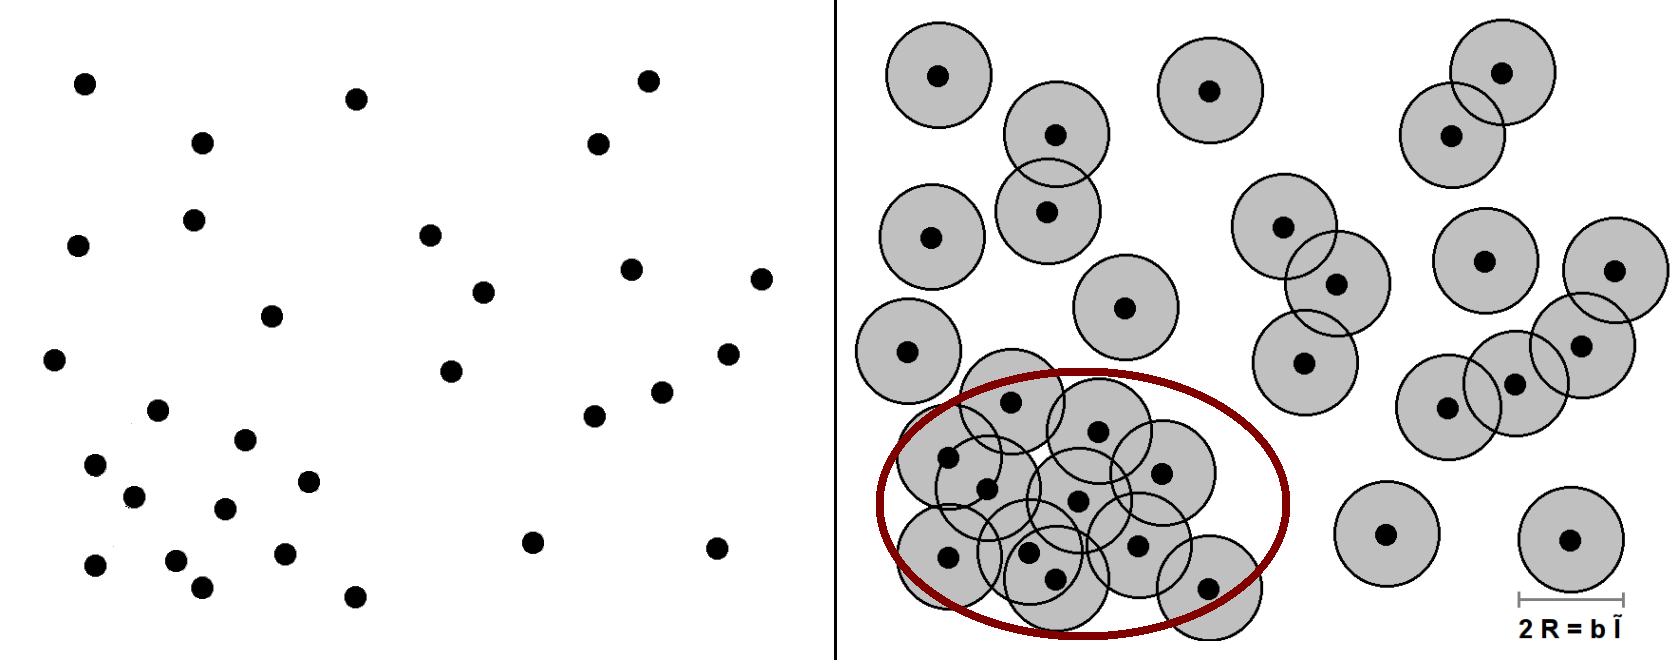
\includegraphics[width=0.9\textwidth]
	{./figures/3_nbody_simulations/FOF_Method.png}

	\caption{\small{Illustrative diagram of the FOF method. Gray circles 
	around each particle represents the linking region and the red curve
	represents one of the bounded structures found by the method.}}
	
	\label{fig:FOF_Method}
\end{figure}
%.........................................................................


%Reviewed
In this method, it is associated a finite volume to each particle which
is called the linking region. Once defined these volumes, the structures
are found by detecting intersections between them. An illustrative example
is shown in the Figure \ref{fig:FOF_Method}, where the structure enclosed 
by the red curve, corresponding to a dark matter halo, is made of the 11
adjacent linking regions which intercept each other. The geometry of the
linking regions is generally spherical, with a radius $R_i$ given by the
next expression


%Reviewed
%.........................................................................
%FOF Diameter
\eq{eq:FOF_Diameter}
{ R_i = \frac{1}{2}b\ \bar l }
%.........................................................................
where $b$ is the linking parameter and $\bar l$ the mean free path of the 
particles of the simulation. The linking parameter $b$ is free and depends
on each simulation particularly, being given a priori before the 
construction of the catalogue of halos.



%Reviewed
Figure \ref{fig:CLUES_FOF} shows the result of applying the FOF method to
construct a catalogue of halos for the CLUES 3 simulation. The distribution
of the halos is in accordance with the density distribution (see Figure 
\ref{fig:TwebVwebComparison}), following the same pattern of filaments and
knots that the cosmic web. In the subsection \ref{subsec:SampleOfPairsToUse}
the defined samples of halos in each simulation are built by using this 
scheme, with a linking parameter $b = 0.17$.


%Reviewed
%.........................................................................
%FOF method in CLUES simulation
\begin{figure}[htbp]
	\centering
	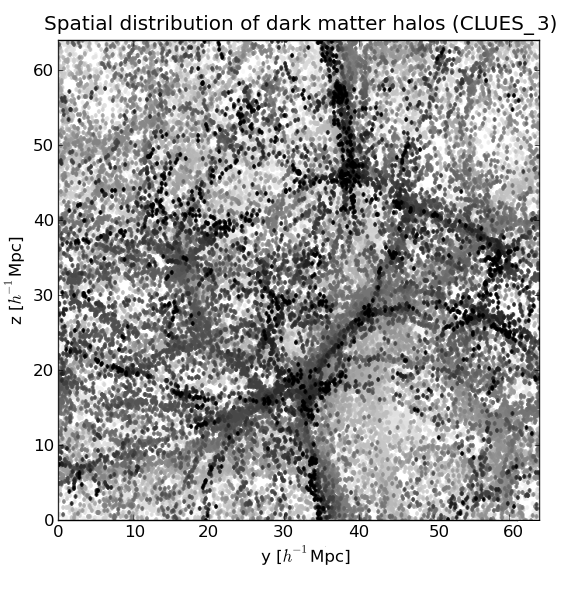
\includegraphics[width=0.5\textwidth]
	{./figures/3_nbody_simulations/Halos_Spatial_Distribution(CLUES_16953).png}

	\caption{\small{Halos detected by using the FOF scheme for one of the 
	CLUES simulations. The color gradient indicates the depth with respect to 
	the	$x$ axe, where black point are the nearest halos.}}
	
	\label{fig:CLUES_FOF}
\end{figure}
%.........................................................................




	%---------------------------------------------------------------------
	%Sample of pairs to use
	\subsection{Defining the Samples}
	\label{subsec:SampleOfPairsToUse}
	%---------------------------------------------------------------------
	

%Reviewed
In this subsection, it is presented the samples that will be used in the 
chapter \ref{cha:Results} for determining the effects of the environment on
LG-like systems and the characterization of each simulation. These samples 
are an extended version of the samples defined by \cite{forero2011}.



%.........................................................................
%Samples in All Simulations
\begin{itemize}
%Reviewed
\item \textbf{General Halos} \textit{(GH)}\textbf{:} these halos correspond
to all halos found in the simulations by using the FOF method, independently
of the mass range.

%Reviewed
\item \textbf{Individual Halos} \textit{(IH)}\textbf{:} they are a subset of
the previous sample and represent all halos that are within the mass range
$5.0 \times 10^{11}\Msun - 5.0\times 10 ^{12}\Msun$. This mass range is 
selected because it corresponds to the range in which disc galaxies form,
such as the main members of the local group, Andromeda and the Milky Way.

%Reviewed
\item \textbf{Pairs} \textit{(P)}\textbf{:} this sample is built from the 
\textit{IH} sample and is composed by all halos that satisfy the criterion
to be the closest neighbour to each other. It is constructed as a primitive
sample in order to find isolated pairs and LG-like systems.


%Reviewed
\item \textbf{Isolated Pairs} \textit{(IP)}\textbf{:} this sample is built
from the systems of the Pair sample which furthermore satisfy the next 
conditions \cite{forero2011} \cite{forero2013}.


%Reviewed
%.........................................................................
%CLG conditions
	\begin{itemize}
	\item The distance between the center of each halo should be less than
	$0.7 h^{-1}$ Mpc, what is consistent with the distance between Andromeda
	and the Milky Way.
	\item The relative radial velocity of the pair system should be negative.
	\item There should be no objects more massive than both halos at a distance
	less than $2.0 h^{-1}$ Mpc with respect to the position of the pair.
	\item There should be no objects more massive than $5.0 \times 10^{13}
	\Msun$ at a distance less than $5h^{-1}$ with respect to both halos.
	\end{itemize}
%.........................................................................	
	

%Reviewed
These conditions guarantee the isolation of the pairs with respect to the
gravitational influence of larger structures and other halos.


%Reviewed
\item \textbf{LG-like Systems} \textit{(LG)}\textbf{:} this sample is 
defined in the CLUES simulations and corresponds to the halo pairs built
a priori for reproducing the local group. By definition, there is only a
\textit{LG} system in each one of three simulations.


%Reviewed
\item \textbf{Constructed Local Groups} \textit{(CLG)}\textbf{:} with the
aim to obtain a \textit{LG}-like sample in unconstrained simulations, it 
is proposed a novel construction method base upon the cosmological 
environment of the \textit{LG} sample previously defined in the CLUES
simulations (see Figure \ref{fig:LG_Sample_Environment}). For this it is
computed the three eigenvalues fields of the shear velocity tensor onto a
grid with a resolution of $1.0 h^{-1}$ Mpc/cell and a Gaussian softening
of one cell size. In the next Table is tabulated the obtained values for 
the eigenvalues of the environment for the \textit{LG}-like systems.


%Reviewed
%.........................................................................
%Table of extreme values of LG environment
\begin{table}[htbp]
\begin{flushright}
\begin{minipage}[r]{0.9\textwidth}
\begin{small}
  \centering
  \begin{tabular}{| c | c | c | c |} \hline
	\cellc{\textbf{Description} }		 				     & 
	\cellc{$\bds{\lambda_{1}}$ \footnotesize{$[10^{-1}]$}}   & 
	\cellc{$\bds{\lambda_{2}}$ \footnotesize{$[10^{-1}]$}}   & 
	\cellc{$\bds{\lambda_{3}}$ \footnotesize{$[10^{-1}]$}}   \\ \hline
	
	{CLUES 1\ H1} & 1.82 		& 1.20 				 	 & -1.59 \\
	{CLUES 1\ H2} & 1.82 		& 1.20 					 & -1.59 \\ \hline
	{CLUES 2 H1} & 1.78 		& 9.54$\times 10^{-1}$   & -8.85$\times 10^{-1}$ \\
	{CLUES 2 H2} & 2.19		& 4.45$\times 10^{-2}$   & -1.29 \\ \hline
	{CLUES 3 H1} & 3.23 		& -6.29$\times 10^{-2}$  & -1.98 \\
	{CLUES 3 H2} & 3.49 		& 1.21 					 & -1.29 \\ \hline
	{Maximum value} & 1.78 	& -6.29$\times 10^{-2}$  & -1.98 \\
	{Minimum value} & 3.49 	& 1.21					 & -8.85$\times 10^{-1}$ \\ \hline
  \end{tabular}
  
  \caption{Eigenvalues associated to the environmental properties of each
  Local Group found in the CLUES simulations.}  
  \label{tab:Lambdas_LG}
\end{small}
\end{minipage}
\end{flushright}
\end{table}
%.........................................................................


%Reviewed
%.........................................................................
%LG Environment in CLUES simulation
\begin{figure}[htbp]
\begin{flushright}
\begin{minipage}[r]{0.9\textwidth}
	\centering
	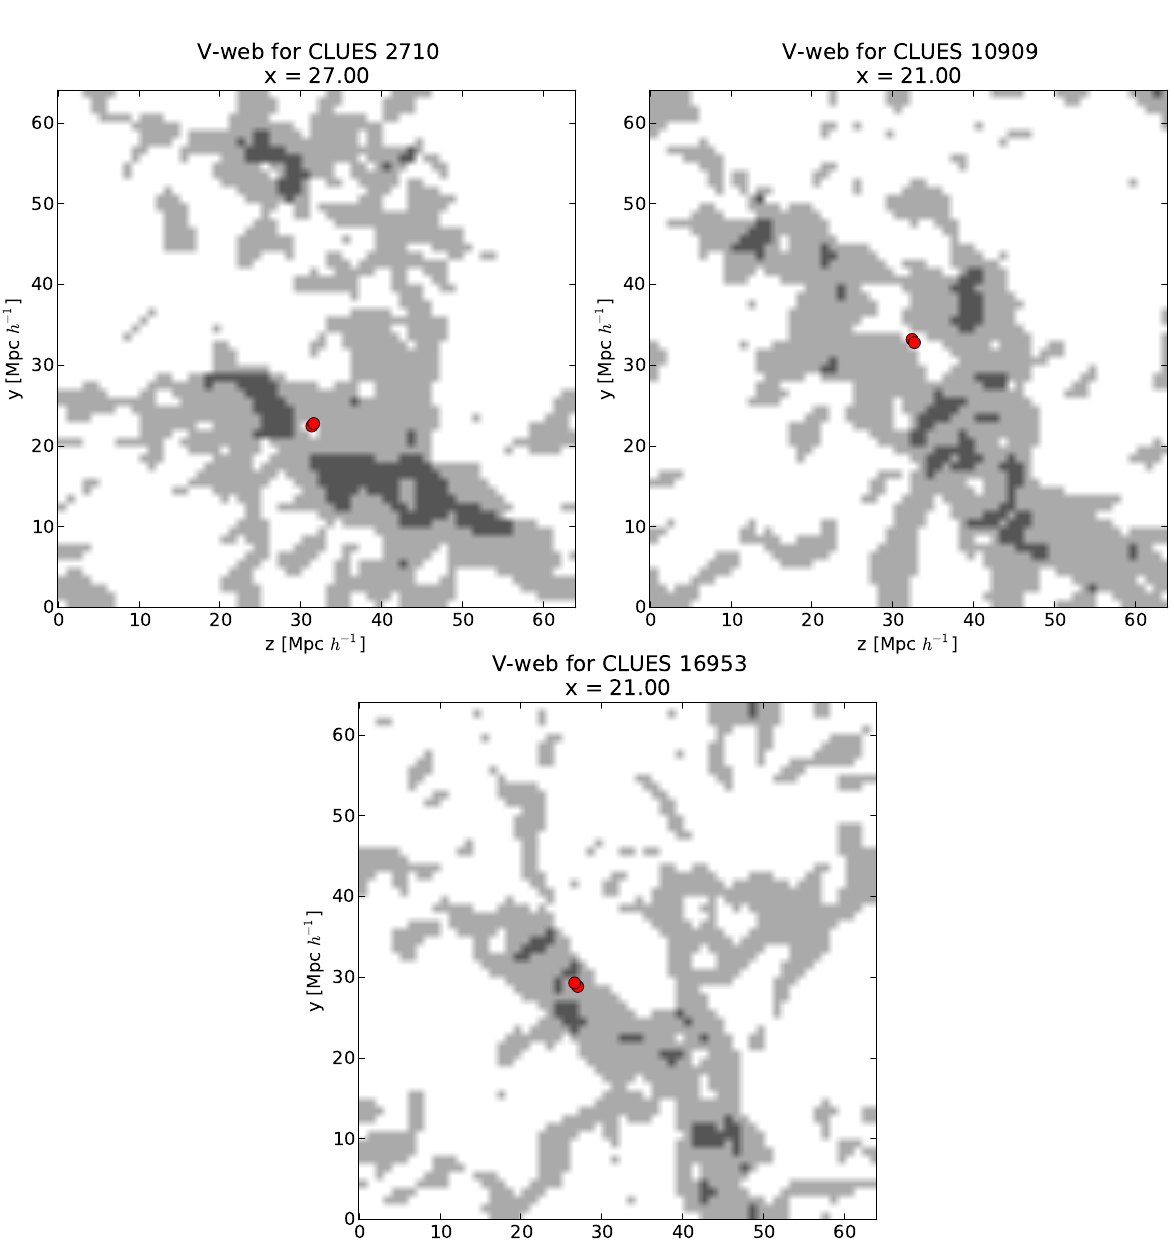
\includegraphics[width=0.75\textwidth]
	{./figures/3_nbody_simulations/LG_Environment.png}

	\caption{\small{Cosmological environment obtained by using the V-web
	scheme (with $\lambda_{th} = 0.3$) for each one of the LG-like systems
	in the CLUES simulations (red dots).}}
	\label{fig:LG_Sample_Environment}
\end{minipage}
\end{flushright}
\end{figure}
%.........................................................................


%Reviewed
Finally, from the extreme values of the eigenvalues previously found, it
is defined the \textit{CLG} sample as all the pairs \textit{IP} whose 
respective eigenvalues are within the set range. In order to guarantee
self-consistency, it is constructed a \textit{CLG} sample in the CLUES
simulations.



\end{itemize}
%.........................................................................


%Reviewed
%.........................................................................
%Table of samples numbers
\begin{table}[htbp]
\begin{small}
  \centering
  \begin{tabular}{| c | c | c | c | c |} \hline
	\cellc{\textbf{Sample}}		& 
	\cellc{\textbf{CLUES 1}}		& 
	\cellc{\textbf{CLUES 2}} 		& 
	\cellc{\textbf{CLUES 3}}		& 
	\cellc{\textbf{Bolshoi}}		 \\ \hline
	\textit{GH} 	& 56632 & 57707 & 56799  & 432000 	\\
	\textit{IH}		& 1493 	& 1490 	& 1493	 & 88068 	\\
	\textit{P}		& 386 	& 380 	& 387	 & 23037 	\\
	\textit{IP}		& 20 	& 12 	& 18 	 & 1256 	\\
	\textit{LG}		& 1 	& 1 	& 1 	 & --		\\
	\textit{CLG}	& 1 	& 2 	& 3 	 & 30		\\ \hline
  \end{tabular}
  
  \caption{Size of the defined samples in each one of the simulations. }  
  \label{tab:Samples}
\end{small}
\end{table}
%.........................................................................


%Reviewed
To finish, in Table \ref{tab:Samples} is tabulated the size of each one
of the defined samples in each simulation. It can be noticed that their 
sizes scale approximately in the same proportion that the volume of the 
simulations ($1/60$ -- CLUES /Bolshoi). Specially, the \textit{CLG} sample 
in Bolshoi has a proportional size that the \textit{LG} in CLUES, thereby
indicating that the proposed construction scheme reproduces LG-like systems
in unconstrained simulations.



	%---------------------------------------------------------------------
	%Sample Detection Method
	\subsection{Method to Detect Pairs}
	\label{subsec:Pairs_Detection}
	%---------------------------------------------------------------------
	

%Reviewed
Next, it shall be described the algorithm developed for detecting each one
of the samples of pair in the simulations (\texttt{Pair Finder}) \footnote{
An updated version of this code can be found in the next github repository
\url{https://github.com/sbustamante/Thesis/tree/master/codes/Halo_Finder}}.



%.........................................................................
%Algorithm of pair finder
\begin{itemize}
%Reviewed
\item It is partitioned the space of the simulation into $N\times N \times
N$ cells, then for each cell it is performed an indexation of the Halos 
within, storing the identification of each one of them.

%Reviewed
\item Next, for each cell it is identified the first neighbours, taking 
into account periodic boundary conditions, such as the cell $i$ in the 
Figure \ref{fig:Pair_Finder}.

%Reviewed
\item For a halo within a given cell, it is calculated the distance to 
all the other halos within the same cell and the neighbour cells, then
it is stored the distance to the closest halo, the distance to the closest
halo with a mass greater than the current mass and finally the distance to 
the closest halo with a mass grater than $5.0 \times 10^{13}\Msun$.

%Reviewed
\item Repeating the previous step for all the halos, if two halos are the
closest to each other, they are catalogued as a pair system, constructing
in that way the \textit{P} sample defined in the previous subsection
\ref{subsec:SampleOfPairsToUse}.

%Reviewed
\item Finally, for each one of the pair systems it is evaluated the 
defining conditions for the \textit{IP} systems, thereby determining 
this sample.
\end{itemize}
%.........................................................................


%Reviewed
%.........................................................................
%Pair Finder Diagram
\begin{figure}[htbp]
	\centering
	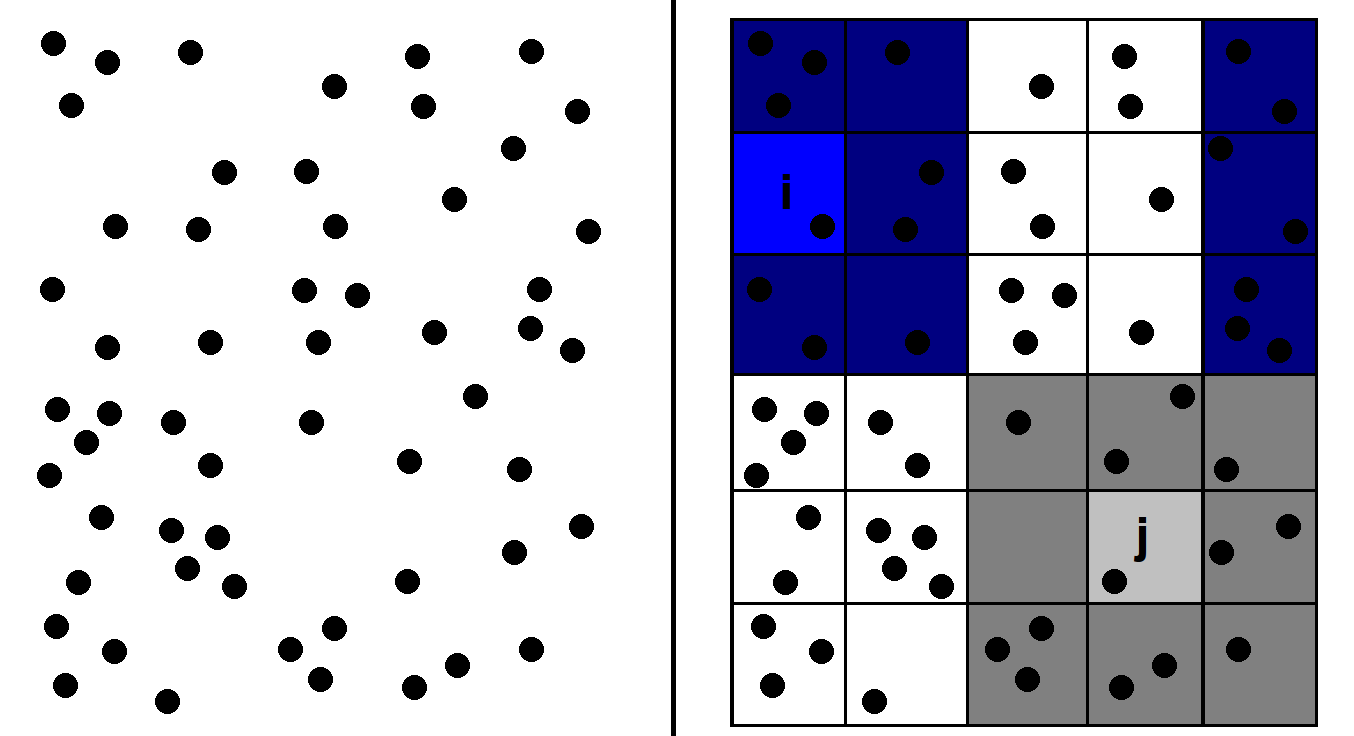
\includegraphics[width=0.6\textwidth]
	{./figures/3_nbody_simulations/PairFinder.png}

	\caption{\small{Two-dimensional of the method for detecting the pair 
	samples. Random distribution of a set of dark matter halos (left), 
	definition of cells (right).}}
	\label{fig:Pair_Finder}
\end{figure}
%.........................................................................


%Reviewed
The efficiency of this method lies in avoiding evaluating distances between
all the halos of the simulations, being only necessary just for the closest
neighbours. The structure of the grid makes this scheme similar to a tree 
code (see subsection \ref{subsec:P3Method}), excepting the hierarchical
structure performed in the latter. At first, this code should be more 
efficient as it is increased the resolution $N$ of the grid, but there are
two limitations to this. First, the number of halos per cell should not
be very large, but neither that there are just a few halos per cell
\footnote{This threshold is not well-defined and depends on each simulation
particularly, for instance for the used simulation (Bolshoi and CLUES), a
value of $N=8$ is generally enough.} The second limitation is related with
the conditions of distance used for defining the \textit{IP} sample, the
physical size of each cell cannot be less than any of these distances.



%*************************************************************************